\documentclass[11pt]{article}
\usepackage[margin=1in]{geometry}
\usepackage{amsmath,amssymb,amsthm}
\usepackage{booktabs,enumitem,xcolor,array,tabularx,graphicx,float}
\usepackage{microtype}
\usepackage[colorlinks=true,linkcolor=blue!50!black,citecolor=blue!50!black,urlcolor=blue!50!black]{hyperref}
\newcolumntype{Y}{>{\raggedright\arraybackslash}X}
\setlength{\emergencystretch}{2em}
\setlength{\parskip}{3pt}
\newtheorem{theorem}{Theorem}
\newcommand{\E}{\mathbb{E}}
\newcommand{\status}[1]{\textcolor{orange!70!black}{\textbf{[#1]}}}
\newcommand{\verdict}[1]{\textcolor{blue!50!black}{\textbf{Verdict: #1}}}
\graphicspath{{figures/}{../paper/figures/}}
\hypersetup{pdftitle={Research report: rollouts, noise, and negative reinforcement in RLVR}}

\title{\textbf{Same Direction, Different Noise}\\[4pt]
\large A research report on rollout collection, gradient noise, and negative reinforcement\\ in reinforcement learning with verifiable rewards}
\author{Mohamed Ayman\\\small Working report, October 17, 2026. Covers everything done so far; items marked \status{running} are still in progress.}
\date{}

\begin{document}
\maketitle

\section*{Summary}

\textbf{The question.} When a language model is trained with reinforcement learning on math problems, it writes several answers per question, each answer is graded right or wrong, and the model is updated. Every design choice in this loop (how many answers to write, which answers to push up or down, and by how much) changes three things at once: which direction the update points, how noisy it is, and how much it costs. We set out to make these effects exact and measurable.

\textbf{What we found, in order.}
\begin{enumerate}[leftmargin=*,itemsep=2pt]
\item \textbf{An exact theorem.} For right-or-wrong rewards, the average update and the noise of \emph{any} answer-collection rule depend on only four numbers per question. This holds even when the number of answers per question is random.
\item \textbf{A new measurement.} In Qwen2.5-Math-1.5B, wrong answers have about 2.5 to 3 times larger squared gradients than right ones, while being only 9\% longer. Nobody had measured this. Two 2026 papers assume the opposite.
\item \textbf{A null result that taught us something.} Using that measurement to scale down wrong answers did not improve training (minus 2.2 and minus 2.7 points in two seeds). Smarter answer-collection rules gave small but consistent gains at equal cost: plus 1.1 and plus 3.3 points for our optimal rule on 3{,}382 held-out problems, plus 2.0 and plus 0.8 for probe-then-fill.
\item \textbf{The main finding.} Rewarding only right answers (PSR) and penalizing only wrong answers (NSR) have \emph{exactly the same average update}. Penalizing wrong answers equals rewarding right answers plus a term whose average is zero, pure noise. Because wrong answers carry larger gradients, NSR is about 6 times noisier (theory about 7, measured 6.4). In our experiments NSR learns more slowly, ends with lower pass@1, and reaches the \emph{same} pass@64 as PSR and Dr.\ GRPO (83.0, 83.2, 83.2 in seed 1). This contradicts the explanation in a NeurIPS 2025 paper that negative samples are special for preserving diversity.
\item \textbf{Our noise formula holds in the real model.} The measured gradient noise matches the theorem within 0 to 30\% for every rule in both seeds.
\end{enumerate}

\textbf{Where we are.} The theory and the noise measurements are solid. The key remaining question is whether NSR has more diversity than PSR \emph{at the same accuracy}. Early data say no, but the data are still within noise. Three pre-registered tests that answer it are running: the same question with two new seeds, the NSR paper's own implementation choices, and a dose-response test across five baselines.

\tableofcontents
\newpage

\section{Background: what we started from}

\textbf{Reinforcement learning with verifiable rewards (RLVR).} For each math question, the model samples a group of $n$ answers. A program checks each final answer (reward 1 if right, 0 if wrong). The model then increases the probability of some answers and decreases others, weighted by an \emph{advantage} $A_i$ per answer. The update is $g=\sum_i A_i\,\nabla\log\pi(y_i)$.

\textbf{GRPO and Dr.\ GRPO.} GRPO sets $A_i=(r_i-\bar r)/\mathrm{std}(r)$ and averages each answer's loss over its tokens. Dr.\ GRPO (``GRPO done right'') removes both divisions, which bias training, so $A_i=r_i-\bar r$. Example: if 2 of 8 answers are right, $\bar r=0.25$, right answers get $+0.75$ and wrong answers get $-0.25$. Dr.\ GRPO is our main baseline.

\textbf{Adaptive answer collection.} Many recent methods decide adaptively how many answers to write per question: DAPO drops questions whose answers all agree and refills the batch; probe-then-fill methods (SPEED-RL, SARA, Pilot-Commit) write a few answers and continue only on questions with mixed results; others sample until a correct answer appears. These rules change the update's direction, noise, and cost at the same time, and they are usually compared by heuristics.

\textbf{The original idea (WORTH).} Make the value of each generated answer exact: derive the direction, noise, and cost of any collection rule, find the optimal rule, and test the predictions in real training.

\section{Theory}

\subsection{The two-moment theorem}
Let $p$ be a question's success probability, $\ell(y)=\nabla\log\pi(y)$ the score of answer $y$, $F_1$ and $F_0$ the mean squared score norms of right and wrong answers, and $\kappa(1)=1/p$, $\kappa(0)=-1/(1-p)$.

\begin{theorem}
For any rule that decides when to stop sampling and which advantages to assign from the rewards seen so far (including random group sizes),
\[
\E g=c(p)\,\nabla p,\qquad \E\|g\|^2=F_1D_1(p)+F_0D_0(p)+\|\nabla p\|^2X(p),
\]
where $c$, $D_1$, $D_0$, $X$ and the expected cost $\E N$ depend only on the rule and $p$.
\end{theorem}
\textbf{Why it is true.} A right answer's average score is $\nabla p/p$ and a wrong answer's is $-\nabla p/(1-p)$. Given the whole sequence of rewards, the stopping time and advantages are fixed numbers and the answers are independent, so averaging over answers and then over rewards gives both formulas. No optional-stopping argument is needed. \textbf{What is new:} the average update for fixed groups was known (Davis and Recht, 2025; ARCUS, 2026); the second moment with separate $F_0$ and $F_1$ and random group sizes is not in the literature we found. The derivation is short; the generality and the measured $F_0\neq F_1$ are the contribution. All statements are verified by exact enumeration in small softmax models (\texttt{theory/exact.py}).

\subsection{Efficiency and the optimal rule}
Treating questions as having unrelated gradients and choosing the step size optimally, the progress in mean accuracy per generated answer is proportional to $\mathrm{Sig}^2/(\mathrm{Cost}\cdot\mathrm{M2})$. Dynamic programming over the lattice of (wrong, right) counts finds the optimal rule. Main conclusions, exact within the model:
\begin{itemize}[leftmargin=*,itemsep=1pt]
\item DAPO's dynamic sampling has exactly the per-answer efficiency of the fixed group it filters, because dropped questions cost their answers and contribute nothing.
\item Sample-until-correct rules are the least efficient.
\item Probe-then-fill is the best rule in use; the optimal rule beats it by 1.3 to 1.7 times, and Dr.\ GRPO by 1.7 to 2.3 times, with the measured inputs.
\end{itemize}

\begin{table}[H]
\centering\small
\begin{tabularx}{\linewidth}{@{}>{\raggedright\arraybackslash}p{0.42\linewidth}YYYY@{}}
\toprule
\textbf{Rule} & \textbf{Uniform} & \textbf{Mostly hard} & \textbf{U-shaped} & \textbf{Mostly easy}\\
\midrule
Fixed group of 8 (GRPO, Dr.\ GRPO, DAPO) & 0.61 & 0.38 & 0.40 & 0.38\\
Fixed group of 16 & 0.65 & 0.41 & 0.43 & 0.41\\
Probe 4, abandon if all agree, fill to 16 & 0.77 & 0.60 & 0.67 & 0.60\\
Sample until 1 correct, cap 16 & 0.26 & 0.09 & 0.12 & 0.30\\
\bottomrule
\end{tabularx}
\caption{Efficiency relative to the optimal rule, by the difficulty mix of the questions.}
\end{table}

\subsection{When does a better rule matter? The critical budget}
Without the assumption that questions have unrelated gradients, the exact one-step progress at $B$ answers per step is $\langle\nabla J,\mu\rangle^2/(2L(s+nV/B))$, with $\mu$ the mean update per question, $s=\|\mu\|^2$, and $V$ its noise. The \emph{critical budget} $B^\star=nV/s$ separates two regimes: below it, a rule with $k$ times the efficiency is worth $k$ times the answers (about $\sqrt k$ under Adam at a fixed learning rate); above it, no rule helps (Figure~\ref{fig:regime}). We later found that this framing is already published for GRPO (Bansal et al., HiLD at ICML 2026), so it is now background, not a contribution.

\begin{figure}[H]
\centering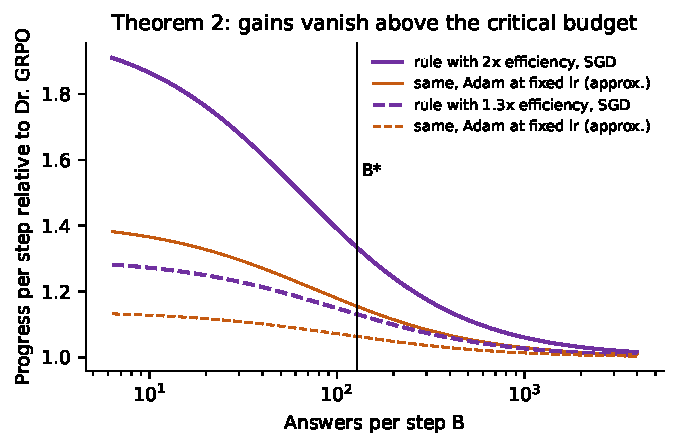
\includegraphics[width=0.55\linewidth]{regime.pdf}
\caption{Predicted gain of a better rule against answers per step. Gains vanish above the critical budget, and Adam at a fixed learning rate turns a gain of $k$ into about $\sqrt k$.}
\label{fig:regime}
\end{figure}

\subsection{Positive and negative reinforcement: same mean, different noise}
Take advantages that depend only on an answer's own reward: $a$ for right, $b$ for wrong. The theorem gives
\[
\E g = n(a-b)\,\nabla p,\qquad \text{noise}\approx n\big(a^2pF_1+b^2(1-p)F_0\big).
\]
\begin{itemize}[leftmargin=*,itemsep=1pt]
\item \textbf{PSR} ($a=1$, $b=0$) and \textbf{NSR} ($a=0$, $b=-1$) both have mean $n\nabla p$: \emph{exactly the same expected update}.
\item In fact $\text{NSR} = \text{PSR} - \sum_i\nabla\log\pi(y_i)$. The extra term has expected value exactly zero (shifting every advantage by a constant), so it is pure noise.
\item PSR's noise is $n\,p\,F_1$ (it lives on easy questions); NSR's is $n(1-p)F_0$ (on hard questions). With $F_0/F_1\approx2.5$, NSR is noisier on every question solved less than 71\% of the time.
\item The whole family $A=r-b$ shares the mean, with noise $n[(1-b)^2pF_1+b^2(1-p)F_0]$, smallest near $b^\star=pF_1/(pF_1+(1-p)F_0)\approx0.15$, well below the group mean that Dr.\ GRPO and RLOO use.
\end{itemize}
\textbf{Consequence.} To first order in the step size, any difference between PSR and NSR (entropy, pass@k, stability) must come from the noise, from an optimizer that reacts to noise (Adam), or from implementation choices outside the theorem (per-token averaging, clipping, stale samples).

\section{Measurements in a real model}

\subsection{Wrong answers carry larger gradients}
We computed exact per-answer gradients in Qwen2.5-Math-1.5B on MATH training problems.
\begin{itemize}[leftmargin=*,itemsep=1pt]
\item Last-layer block, 40 questions by 16 answers: $F_1/F_0=0.36$ (90\% intervals do not overlap), while wrong answers are only 9\% longer (421 vs 386 tokens).
\item All 1.5B parameters, calibration before each training run: $F_1/F_0$ between 0.32 and 0.42 across runs, so wrong answers carry 2.4 to 3.1 times larger squared gradients.
\item Likely reason: wrong answers contain more low-probability tokens, whose scores are large.
\end{itemize}
This contradicts Assumption B.3 of VSR (Wang, Liu, Wang, October 2026: ``the expected squared score-function norm does not depend on the realized reward'') and an approximation in BICC (2026).

\subsection{Gradient signal against difficulty}
With 96 answers per question in the last-layer MLP, the unbiased estimate of $\|\nabla p\|^2$ is $0.73\pm0.60$ on very easy or very hard questions and $15.5\pm5.4$ on medium ones (Figure~\ref{fig:shape}). The signal fades at both ends, best fit $p^2(1-p)^2$.

\begin{figure}[H]
\centering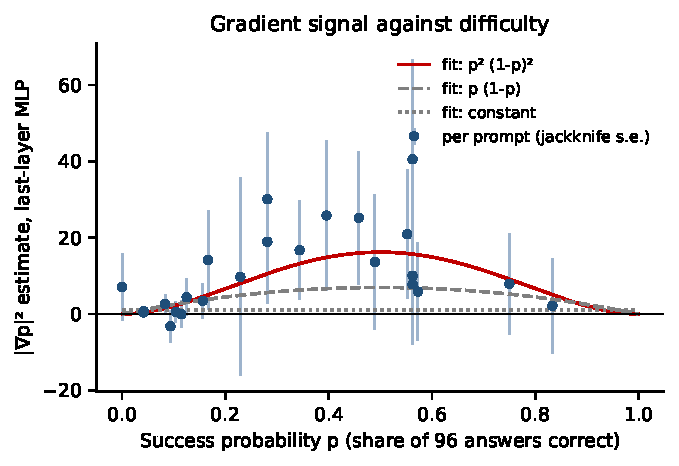
\includegraphics[width=0.55\linewidth]{shape.pdf}
\caption{Per-question gradient signal against success probability, with fits of three shapes.}
\label{fig:shape}
\end{figure}

\subsection{Measuring noise inside training}
At every training step we split the questions into two random halves and record the inner products of the two halves' gradients and of each half with an independent unbiased reference for the population gradient. This gives, per step and without extra sampling, the mean update's size, its noise, and the noise scale. Two results:
\begin{itemize}[leftmargin=*,itemsep=1pt]
\item \textbf{The noise formula holds in the real model.} For every rule, the measured per-question second moment divided by the theorem's prediction is between 0.68 and 1.00 (Figure~\ref{fig:noise}), inside the pre-registered 30\% tolerance for all eight main runs.
\item \textbf{Training becomes more noise-limited as it plateaus.} Dr.\ GRPO's noise scale grows from about 900 answers (steps 0 to 49) to over 10{,}000 (steps 50 to 149) in both seeds: the shared signal shrinks while the noise does not.
\end{itemize}

\begin{figure}[H]
\centering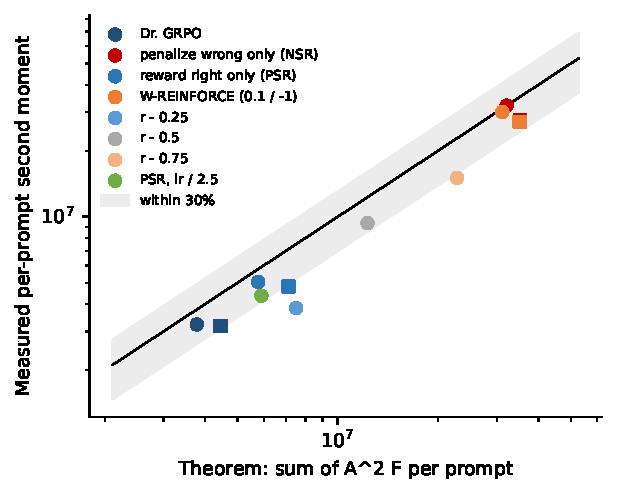
\includegraphics[width=0.5\linewidth]{noise_validation.pdf}
\caption{Measured per-question gradient second moment (steps 0 to 49) against the theorem's prediction from $F_0$, $F_1$ and the observed reward counts. Circles: odd seeds; squares: even seeds. Shaded: within 30\%. The dose-response runs (B25, B50, B75, PSRlow) have few steps so far.}
\label{fig:noise}
\end{figure}

\section{Experiments}
All experiments use Qwen2.5-Math-1.5B base, 3{,}920 numeric MATH training problems, strictly on-policy updates with sequence-sum losses, AdamW at $10^{-6}$, 16 questions by 8 answers per step (128 answers), and 150 steps, unless stated. Every experiment was pre-registered (\texttt{experiments/training/PREREGISTRATION\_*.md}) before its runs started. Evaluation: greedy accuracy on the 364 numeric MATH-500 problems, sampled accuracy and pass@k, and in later runs a 3{,}382-problem held-out MATH set.

\subsection{Pilot: scale down wrong answers (Pre-registration 1)}
\textbf{Why.} With $F_0>F_1$, the theory says to weight a wrong answer by about $F_1/F_0$, a one-line change to GRPO predicted to raise efficiency by 1.1 to 1.6 times.
\textbf{Result.} No gain: 45.3\% vs 47.5\% (seed 1) and 44.0\% vs 46.7\% (seed 2). Training reward was slightly higher early, then tied (Figure~\ref{fig:pilot}). \verdict{no evidence.}
\textbf{Lesson.} Under Adam at a fixed learning rate, the predicted 1.1 to 1.6 times shrinks to 1.06 to 1.25 times, too small to see in two seeds.

\begin{figure}[H]
\centering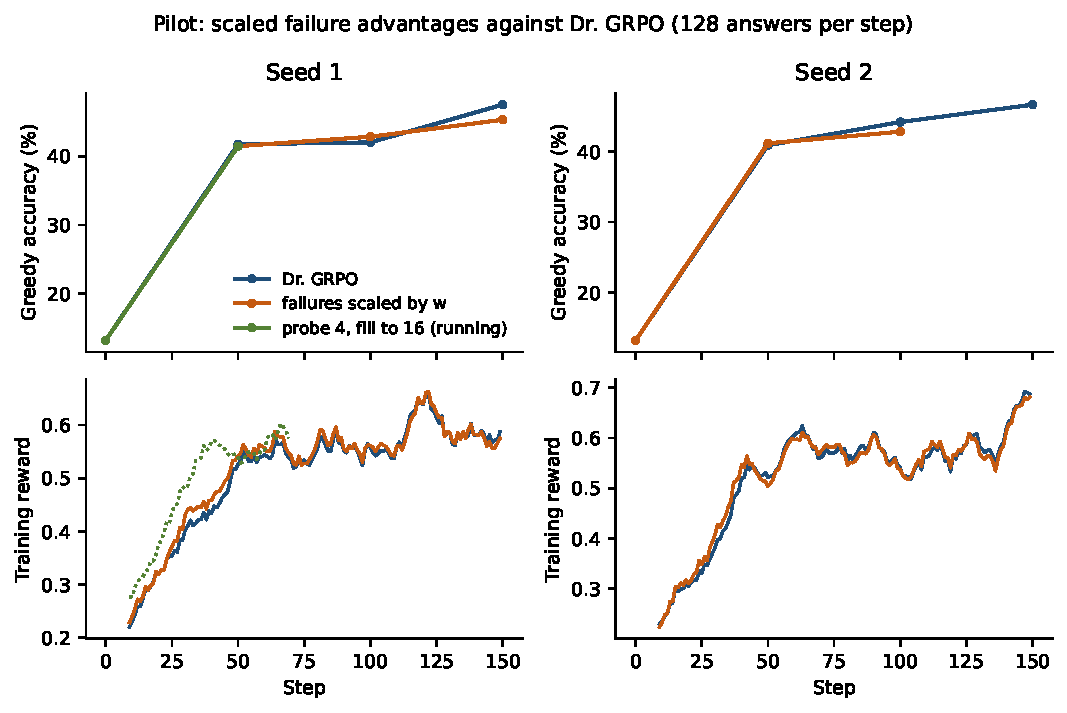
\includegraphics[width=0.85\linewidth]{pilot.pdf}
\caption{Pilot. Top: greedy accuracy. Bottom: training reward. Scaled failures (orange) track Dr.\ GRPO (blue). Probe-then-fill (green) is dotted because its training reward weights questions differently.}
\label{fig:pilot}
\end{figure}

\subsection{Answer-collection rules at equal cost (Pre-registrations 2 and 3)}
\textbf{Why.} Test the optimal rule and probe-then-fill at exactly matched generated answers (19{,}200), with paired per-problem comparisons on the 3{,}382-problem set.
\begin{table}[H]
\centering\small
\begin{tabular}{@{}lcc@{}}
\toprule
\textbf{Run (versus Dr.\ GRPO at 128 answers per step)} & \textbf{Seed 1} & \textbf{Seed 2}\\
\midrule
Optimal rule, 128 answers per step (paired, 3{,}382 problems) & $+1.1\pm0.4$ & $+3.3\pm0.5$\\
Scaled failures (paired, 3{,}382 problems) & $-0.4\pm0.4$ & $+1.1\pm0.4$\\
Dr.\ GRPO with 32 answers per step (paired, 3{,}382 problems) & $-4.4\pm0.5$ & not run\\
Probe-then-fill (MATH-500 greedy, against the pilot's Dr.\ GRPO) & $+2.0$ & $+0.8$\\
\bottomrule
\end{tabular}
\caption{Accuracy differences in points (standard errors for paired comparisons).}
\end{table}
\textbf{Reading.} The optimal rule gains in both seeds, $+1.1\pm0.4$ and $+3.3\pm0.5$ (2.7 and 6.6 standard errors), with matched answers (19{,}172 and 19{,}200) and about 1\% more tokens. The strict pre-registered rule (at least 1.5 points in both seeds) is not met because seed 1 falls short. Probe-then-fill is positive in both seeds. Gains are much smaller than the one-step theory predicts, consistent with Adam's square-root effect. Fewer answers per step clearly hurts (32 vs 128: minus 4.4 points).

\subsection{Literature review and change of direction}
Three literature reviews (verified by hand on the key papers) found:
\begin{itemize}[leftmargin=*,itemsep=1pt]
\item \textbf{The critical-budget framing is taken:} Bansal, Mohri, Abreu, Alvarez-Melis, Kakade, ``Critical Batch Size for LLM Policy Optimization'' (HiLD at ICML 2026) decomposes GRPO noise into between-question and within-question terms and finds the within-question term dominant, as our measurements do. Li et al.\ (arXiv 2608.29296) show square-root learning-rate scaling; IsoCompute (arXiv 2603.12151) studies answers per question.
\item \textbf{Common flaws in adaptive-rollout papers:} gains plotted against training steps while spending 2 to 3 times more answers per step (for example, SARA's plus 6.8 points comes with 3.3 times the answers), learning rate not retuned, single seeds, 30-problem benchmarks, best checkpoints chosen on the test set, mechanisms (``lower variance'') never measured.
\item \textbf{Nobody measures gradient norms by correctness}, and no paper separates the mean and the noise of positive and negative reinforcement.
\end{itemize}
So we moved the main question to positive versus negative reinforcement, where our theorem and measurement are unique.

\subsection{PSR, NSR, Dr.\ GRPO and W-REINFORCE (Pre-registration 4)}
\textbf{Why.} Zhu et al.\ (NeurIPS 2025) report that training only on negative samples (NSR) preserves entropy and pass@k while positive-only training (PSR) collapses them, and recommend W-REINFORCE (weight 0.1 on right answers, $-1$ on wrong). Our theorem says PSR and NSR have identical average updates, so any difference must come from noise or implementation.
\textbf{Design.} Four rules, two seeds, strictly on-policy, with in-training noise measurements, an on-policy entropy probe (the first four answers of every question, the same for all rules), and pass@k with 64 samples per problem at step 150.

\begin{table}[H]
\centering\small
\resizebox{\linewidth}{!}{\begin{tabular}{@{}lcccc@{}}
\toprule
\textbf{Rule} & \textbf{Train acc., steps 25 to 49} & \textbf{pass@1 at 150} & \textbf{pass@64 at 150} & \textbf{Entropy, 100 to 150}\\
& seed 1 / seed 2 & seed 1 / seed 2 & seed 1 / seed 2 & seed 1 / seed 2\\
\midrule
Dr.\ GRPO & 50.6 / 48.0 & 43.3 / 43.2 & 83.2 / 81.9 & 0.227 / 0.224\\
PSR (reward right only) & 51.3 / 48.2 & 42.4 / 42.0 & 83.2 / 83.8 & 0.227 / 0.226\\
NSR (penalize wrong only) & 33.6 / 36.4 & 37.7 / 39.1 & 83.0 / 82.1 & 0.251 / 0.251\\
W-REINFORCE & 38.6 / 38.0 & 38.5 / 39.8 & 80.5 / 81.3 & 0.243 / 0.256\\
\bottomrule
\end{tabular}}
\caption{Main comparison. The untrained model has pass@1 13.8 and pass@64 79.9.}
\end{table}

\begin{figure}[H]
\centering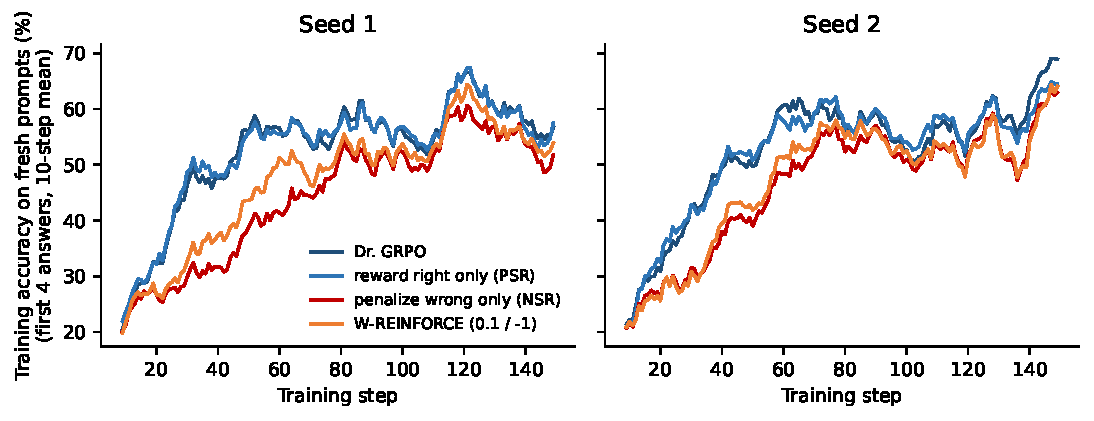
\includegraphics[width=0.95\linewidth]{pn_curves.pdf}
\caption{Training accuracy on fresh questions (unbiased for every rule). NSR and W-REINFORCE, whose updates are dominated by wrong answers, learn clearly more slowly.}
\label{fig:curves}
\end{figure}

\begin{figure}[H]
\centering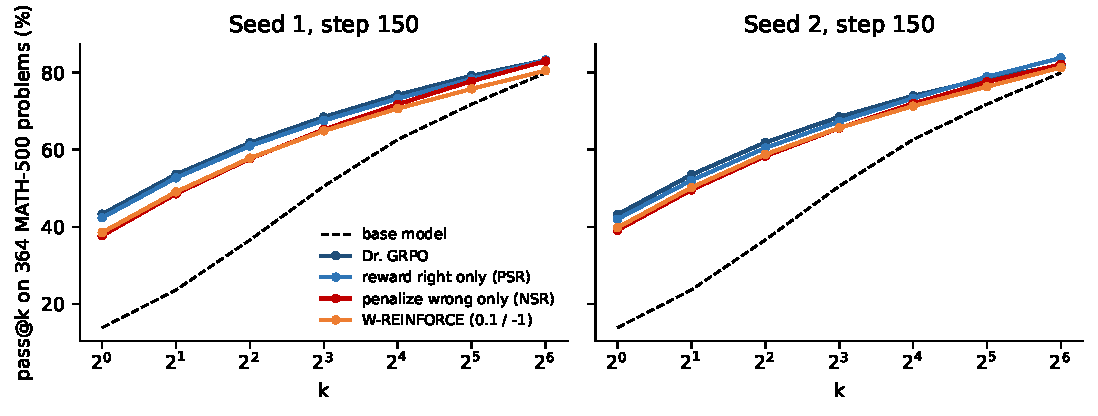
\includegraphics[width=0.95\linewidth]{passk.pdf}
\caption{pass@k at step 150 against $k$. All rules converge at large $k$; NSR and W-REINFORCE are lower at small $k$.}
\label{fig:passk}
\end{figure}

\textbf{Results.}
\begin{itemize}[leftmargin=*,itemsep=1pt]
\item \textbf{Noise:} NSR's measured per-question noise is 6.4 times PSR's (theory about 7).
\item \textbf{Speed:} NSR and W-REINFORCE learn more slowly (Figure~\ref{fig:curves}) and end with 4 to 5 points lower pass@1.
\item \textbf{Diversity:} pass@64 is the same for PSR, NSR and Dr.\ GRPO in seed 1 (83.2, 83.0, 83.2); W-REINFORCE is lower (80.5, 81.3). NSR's entropy is 11\% higher than PSR's.
\item \textbf{Equal-mean check:} the projection of each rule's mean update on the population gradient is too noisy to test (90\% intervals include both 1 and 0).
\end{itemize}
\verdict{the pre-registered separation (at least 3 points of pass@64 or 20\% more entropy in favor of NSR) is not met in either seed: NSR minus PSR pass@64 is $-0.2$ and $-1.7$, and NSR's entropy is 1.11 times PSR's in both seeds.}

\subsection{Equal accuracy, equal diversity? (Pre-registration 5) \status{running}}
\textbf{Why.} If NSR is just a slower PSR, its higher entropy reflects less progress. The decisive test compares diversity at the \emph{same} pass@1: for each NSR checkpoint, PSR's pass@32 at the same pass@1 is interpolated along PSR's trajectory.
\textbf{So far} (pass@32 on 128 problems, noise about $\pm2$ to 3 points per point): seed 3, NSR is 2.8, 3.2, 0.7 and 2.1 points \emph{below} PSR's frontier (mean $-2.2$); seed 4, 3.2, 1.0 and 0.7 points above (mean $+1.6$). The seeds disagree and the average is near zero, consistent with ``same frontier, slower'' and not with ``negative samples add diversity'' (Figure~\ref{fig:frontier}, left).

\begin{figure}[H]
\centering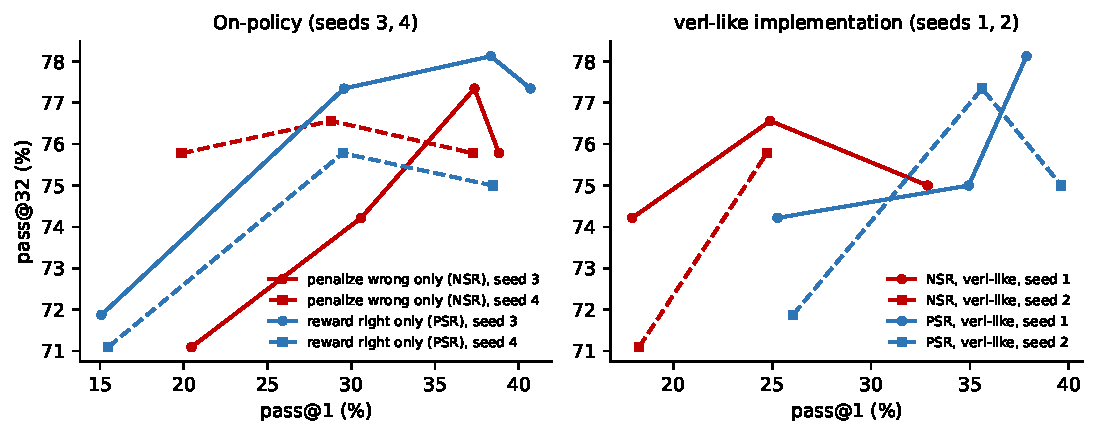
\includegraphics[width=0.95\linewidth]{frontier.pdf}
\caption{Accuracy against diversity during training (pass@1 against pass@32, 128 problems). Left: on-policy. Right: the NSR paper's implementation choices. Points are evaluations at steps 25, 50, 75, 100, 150 (step 0 in PSR runs).}
\label{fig:frontier}
\end{figure}

\subsection{The NSR paper's implementation choices (Pre-registration 6) \status{running}}
\textbf{Why.} Zhu et al.\ used verl, which differs from our setting in three ways the theorem does not cover: each rollout batch is reused for 4 updates with PPO clipping (stale samples), each answer's loss is averaged over its tokens, and PSR and NSR average over only the answers they train on. We reproduce all three at matched answers and updates; with fresh samples our clipped loss equals the plain loss exactly (difference 0.0).
\textbf{So far.} NSR learns even more slowly in this setting (training accuracy 31.0 and 31.4 vs 43.0 and 45.4 over steps 25 to 49), and its checkpoints sit below PSR's pass@1 range, so the matched comparison needs later points (Figure~\ref{fig:frontier}, right).

\subsection{Dose-response across baselines (Pre-registration 7) \status{running}}
\textbf{Why.} The strongest test of ``only noise differs'': advantages $A=r-b$ for $b=0,0.25,0.5,0.75,1$ share the mean exactly, while the theory predicts noise of $1\times$, $0.93\times$, $1.7\times$, $3.4\times$ and $6\times$ PSR's. If outcomes follow this ordering, noise is the cause. A PSR run with the learning rate divided by 2.5 tests the ``slower clock'' reading: it should look like NSR.
\textbf{So far.} Runs are at step 25 to 50, too early to judge; the first training accuracies are in the predicted order (for example $b=0.75$ below $b=0.25$). Verified: $b=0$ reproduces PSR and $b=1$ reproduces NSR exactly.

\section{Discussion}

\textbf{What we have learned.}
\begin{enumerate}[leftmargin=*,itemsep=2pt]
\item In clean on-policy training, how you score right and wrong answers matters mainly through \emph{noise}, and the noise is predictable from four numbers per question.
\item Wrong answers dominate the noise, because their gradients are 2.5 to 3 times larger.
\item Penalizing wrong answers alone does not preserve diversity in our setting; it learns more slowly and reaches the same pass@64.
\item Smarter answer collection helps at equal cost: our optimal rule gains 1.1 and 3.3 points in two seeds, less than one-step theory predicts. Adam's response to noise is the likely reason the gain is smaller.
\end{enumerate}

\textbf{How confident should we be?}
\begin{itemize}[leftmargin=*,itemsep=1pt]
\item \textbf{Strong:} the theorem (exact); the gradient asymmetry (measured two ways, all runs); the noise formula (within 30\% in 8 of 8 main runs); NSR's slower learning (both seeds).
\item \textbf{Moderate:} equal pass@64 (two seeds; NSR is 0.2 and 1.7 points below PSR).
\item \textbf{Open:} equal diversity at equal accuracy (two seeds disagree, within noise); whether the NSR paper's implementation recreates its effect.
\end{itemize}

\textbf{Threats to validity.}
\begin{itemize}[leftmargin=*,itemsep=1pt]
\item \textbf{One model family.} Qwen2.5-Math gains 21 points on MATH-500 even from random rewards (Spurious Rewards, 2025), so small effects on it are suspect; a second family is needed.
\item \textbf{Short training.} 150 steps move pass@64 only from 79.9 to about 82 to 83, which leaves little room for differences.
\item \textbf{Evaluation noise.} pass@32 on 128 problems carries about $\pm2$ to 3 points; the final runs will use all 364 problems.
\item \textbf{Answers counted, not reasoning.} A right final answer can come from wrong reasoning; CoT-Pass@k (Section~\ref{sec:next}) addresses this.
\item \textbf{Theory scope.} One-step, SGD-based progress; the Adam statement is an approximation.
\end{itemize}

\textbf{Engineering issues fixed along the way.} GPU out-of-memory during evaluation (gradients kept alive; fixed by freeing them after each update, training unchanged), crashes on long held-out prompts (batch size now capped by prompt length; the final-check number and saved models were lost for Pre-registration 4), Hugging Face rate limits on shared AWS addresses (model now loaded from our S3 copy), and a grader crash on a sampled \verb|\boxed{1/0}| (fixed and tested). Each fix was verified locally before relaunch.

\section{Next steps}\label{sec:next}
\textbf{1. Finish the explanation.} Collect the three running tests and apply their pre-registered verdicts. Then one high-precision run set (Dr.\ GRPO, PSR, NSR, two new seeds) with pass@32 on all 364 problems, saved answer texts and saved models. Grade the reasoning of every correct answer with an LLM judge (Claude Haiku 5.5 on Bedrock, three judgments each; tested: it accepts correct solutions and rejects a right answer reached by wrong reasoning) and report \textbf{CoT-Pass@k} (Wen et al., 2025): pass@k counting only answers whose reasoning is also correct.

\textbf{2. Then a method.} The explanation suggests that diversity comes from the objective (which questions the update aims at), not from noise. A candidate method, WORTH-k: for a chosen target (pass@1, pass@8, pass@32), use the theory to build the update that aims exactly at it with the least noise per generated answer, accounting for the 2.5 to 3 times gradient asymmetry and for adaptive sampling. Its predicted advantage over existing pass@k methods will be computed with the exact theory before any GPU run.

\appendix
\section{Pre-registrations and verdicts}
\begin{table}[H]
\centering\small
\begin{tabularx}{\linewidth}{@{}lYl@{}}
\toprule
\textbf{\#} & \textbf{Question} & \textbf{Verdict}\\
\midrule
1 & Scaled failure advantages beat Dr.\ GRPO? & No evidence ($-2.2$, $-2.7$)\\
2 & Optimal rule and probe-then-fill at matched answers? & Probe $+2.0$, $+0.8$; optimal replaced by 3\\
3 & Budget ladder, in-training noise, optimal rule at 128 & Optimal $+1.1\pm0.4$, $+3.3\pm0.5$; rule not met\\
4 & PSR vs NSR vs Dr.\ GRPO vs W-REINFORCE & Separation not reproduced (both seeds)\\
5 & Equal diversity at equal pass@1 (seeds 3, 4) & Running; so far $-2.2$ and $+1.6$\\
6 & NSR paper's implementation choices & Running\\
7 & Baseline dose-response and slower-clock control & Running\\
\bottomrule
\end{tabularx}
\end{table}

\section{Compute}
About 118 GPU-instance hours on finished SageMaker jobs (single L40S GPUs, a mix of spot and on-demand), roughly \$480 by our price estimates; the 16 running jobs will add a few hundred dollars. All code, pre-registrations, results, and figures are in the repository \texttt{github.com/mayman150/rlvr-adaptive}.

\end{document}
